% !TeX TS-program = xelatex

\documentclass[compress, 8pt]{beamer}

\usepackage{presentationtemplate}
\usepackage[askip=3mm, bskip=3mm]{terminal}
\usepackage[linenosfontsize=\tiny, askip=3mm, bskip=3mm]{mylisting}
\usepackage{tcolorbox}
\usepackage{tikz}
\usetikzlibrary{positioning}
\usetikzlibrary{shapes.arrows}

\newtcolorbox{task}{
    colback=yellow!50!white,
    boxrule=0.02cm,
    colframe=black,
    sharp corners,
    left=0mm,
    right=0mm,
    top=0mm,
    bottom=0mm,
    before upper={\textbf{Задание}:\:},
}

\title{Приведения типов}

\begin{document}

\frame[plain]{\titlepage}

\begin{frame}[fragile]

    \frametitle{Неявные приведения}

    \hfill\break
    В C++ есть возможность использовать переменные разных типов в одном выражении.
    При этом арифметические и логические операторы ожидают, что их операнды будут
    одинаковых типов.

    \begin{myinplacelisting}[minted language=cpp]
auto a = 1U + 2L;
    \end{myinplacelisting}

    Как вычислить результат такого выражения?
    Тип \verb|1U| --- \verb|unsigned int|\footnotemark{}, а \verb|2L| ---
    \verb|long int|.
    Эти типы могут иметь разный размер и разное представление в памяти.

    \footnotetext{\url{https://en.cppreference.com/w/cpp/language/integer\_literal}}

    \hfill\break
    Эта проблема решается \textbf{неявным приведением}\footnotemark{} типов
    (implicit conversions).
    Суть этого действия заключается преобразовании одного из операндов таким образом,
    чтобы оба операнда имели одинаковый тип.

    \hfill\break
    Приведения бывают \textbf{сужающими} (narrowing conversions) и \textbf{повышающими}
    (promotions).

    \footnotetext{\url{https://en.cppreference.com/w/cpp/language/implicit\_conversion}}

\end{frame}

\begin{frame}[fragile]

    \frametitle{Повышающие преобразования}

    \begin{itemize}

        \item Интегральные типы могут быть повышены до типов большего размера:
            \verb|char| \rightarrow \verb|int|,
            \verb|unsigned int| \rightarrow \verb|unsigned long|
            и т.д.

        \item Типы с плавающей точкой могут быть повышены до типов большей точности:
            \verb|float| \rightarrow \verb|double|.

        \item Тип \verb|bool| повышается до \verb|int|:
            \verb|true| \rightarrow \verb|1|, \verb|false| \rightarrow \verb|0|.

    \end{itemize}

    \hfill\break
    \centering

    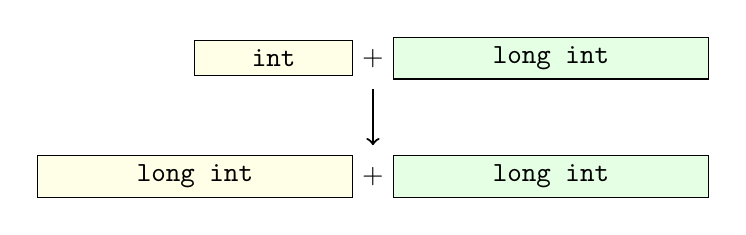
\begin{tikzpicture}

        \matrix[align=right] (before) [column sep=0cm] {
            \node[minimum width=2cm] (fill) {}; &
            \node[draw, minimum width=2cm, fill=yellow!10] (beforeint) {\verb|int|}; &
            \node(beforeplus) {+}; &
            \node[draw, minimum width=4cm, fill=green!10] (beforelong) {\verb|long int|}; \\
        };

        \matrix[below=1.5cm of before.east, anchor=east, align=right] (after) [column sep=0cm] {
            \node[draw, minimum width=4cm, fill=yellow!10] (afterint) {\verb|long int|}; &
            \node(afterplus) {+}; &
            \node[draw, minimum width=4cm, fill=green!10] (afterlong) {\verb|long int|}; \\
        };

        \draw[->, thick] (before.south) -- (after.north);

    \end{tikzpicture}

\end{frame}

\begin{frame}[fragile]

    \frametitle{Сужающие преобразования}

    \begin{columns}[T]

        \begin{column}{0.5\textwidth}

            \myinputlisting[minted language=cpp]
                {Presentations/10-Conversions/narrowing-conversion/}
                {main.cpp}

        \end{column}

        \begin{column}{0.5\textwidth}

            \begin{terminalwindow}
!\shellcommand{g++ main.cpp}!
!\shellcommand{./a.out}!
1
1
4464
            \end{terminalwindow}

            Преобразования между типами, в результате которых теряется информация,
            называются сужающими.

            \hfill\break
            Сужающие преобразования очень часто являются
            \textit{неопределенным поведением}\footnote{\url{https://github.com/Nekrolm/ubbook/blob/master/numeric/narrowing.md}}.

        \end{column}

    \end{columns}

\end{frame}

\begin{frame}[fragile]

    \frametitle{Сужающие преобразования}

    Детектировать сужающие преобразования можно с использованием флагов компилятора.

    \myinputlisting[minted language=cpp]
        {Presentations/10-Conversions/narrowing-conversion-warning/}
        {main.cpp}

    \begin{terminalwindow}
!\shellcommand{g++ -Wconversion main.cpp}!
main.cpp: In function ‘int !\textcolor{teal}{main}!()’:
main.cpp:2:19: !\textcolor{orange}{warning}!: conversion from ‘double’ to ‘int’ changes value from ‘3.5e+0’ to ‘3’ [!\textcolor{orange}{-Wfloat-conversion}!]
    2 |     const int x = !\textcolor{orange}{3.5}!;
      |                   !\textcolor{orange}{\^{}~~}!
    \end{terminalwindow}

\end{frame}

\begin{frame}[fragile]

    \frametitle{Сужающие преобразования}

    \hfill\break
    Потеря информации может происходит при преобразовании из беззнакового типа
    в знаковый.

    \myinputlisting[minted language=cpp]
        {Presentations/10-Conversions/narrowing-sign-conversion-warning/}
        {main.cpp}

    \begin{terminalwindow}
!\shellcommand{g++ -Wsign-conversion main.cpp}!
main.cpp: In function ‘int !\textcolor{teal}{main}!()’:
main.cpp:6:29: !\textcolor{orange}{warning}!: conversion to ‘int’ from ‘unsigned int’ may change the sign of the result [!\textcolor{orange}{-Wsign-conversion}!]
    6 |     const int x = !\textcolor{orange}{get\_number}!();
      |                   !\textcolor{orange}{~~~~~~~~~~\^{}~}!
    \end{terminalwindow}

\end{frame}

\begin{frame}[fragile]

    \frametitle{Сужающие преобразования}

    List-initialization запрещает сужающие преобразования.

    \myinputlisting[minted language=cpp]
        {Presentations/10-Conversions/list-init-narrowing-conversion/}
        {main.cpp}

    \begin{terminalwindow}
!\shellcommand{g++ main.cpp}!
main.cpp: In function ‘int !\textcolor{teal}{main}!()’:
main.cpp:2:19: !\textcolor{red}{error}!: narrowing conversion of ‘3.5e+0’ from ‘double’ to ‘int’ [!\textcolor{red}{-Wnarrowing}!]
    2 |     const int x { !\textcolor{red}{3.5}! };
      |                   !\textcolor{red}{\^{}~~}!
    \end{terminalwindow}

\end{frame}

\begin{frame}[fragile]

    \frametitle{Приведения ссылочных типов}

    \hfill\break
    \begin{itemize}

        \item Любой указатель (кроме указателя на функцию) может быть приведен
            к типу \verb|*|:

            \begin{myinplacelisting}[minted language=cpp]
const int x {};
const void* p = &x;
            \end{myinplacelisting}

        \item Константное выражение, при вычислении которого получается \verb|0|,
            можно привести к указателю любого типа:

            \begin{myinplacelisting}[minted language=cpp]
int* p = 0;
            \end{myinplacelisting}

            Предпочтительно пользоваться \verb|nullptr|.

        \item Любой указатель (ссылка) на тип \verb|T| может быть неявно приведен
            к указателю (ссылке) на тип \verb|const T|:

            \begin{myinplacelisting}[minted language=cpp]
int x {};
int* pointer { &x };
const int* const_pointer { pointer };
int& ref { x };
const int& const_ref { ref };
            \end{myinplacelisting}

    \end{itemize}

\end{frame}

\begin{frame}[fragile]

    \frametitle{Приведения к \texttt{bool}}

    Указатель и объекты арифметических типов могут быть неявно приведены к
    \verb|bool|.
    Объекты, равные \verb|0| приводятся к \verb|false|, все остальные --- к \verb|true|.

    \begin{myinplacelisting}[minted language=cpp]
const int x { 100 };
if (x) {
    // always true
}

const int* const p {};
if (!p) {
    // always true
}
    \end{myinplacelisting}

\end{frame}

\begin{frame}[fragile]

    \frametitle{Неявные приведения}

    \hfill\break
    \begin{task}
        Найдите ошибку, связанную с неявными преобразованиями, в коде на листинге
        ниже.
        Предложите исправление ошибки.
    \end{task}

    \begin{myinplacelisting}[minted language=cpp]
#include <cstddef>
#include <iostream>

double average(const int* const arr, std::size_t size) {
    int sum {};
    for (std::size_t i = 0; i < size; ++i) {
        sum += arr[i];
    }
    return sum / size;
}

int main() {
    const int arr[] = {2, -4, 1};
    std::cout << average(arr, 3) << std::endl;
}
    \end{myinplacelisting}

\end{frame}

\begin{frame}[fragile]

    \frametitle{Явные преобразования}

    Программист может указать компилятору, какое приведение типов он желает получить
    в выражении.
    Такое преобразование будет являться \textbf{явным}.
    Это возможно сделать одним из следующих способов:

    \begin{itemize}
        \item при инициализации объекта с list-initialization \verb|{}|;
        \item с помощью \textbf{именованных преобразований} (named conversions),
            таких как \verb|static_cast|, \verb|const_cast| и др.;
        \item C-style преобразование.
    \end{itemize}

\end{frame}

\begin{frame}[fragile]

    \frametitle{Явные преобразования с list-initialization}

    Рекомендованный вид преобразования, который сочетает в себе безопасность
    и компактность синтаксиса.

    \begin{myinplacelisting}[minted language=cpp]
void foo(const int i, const double d) {
    {
        const int x = i; // ok
        const int y = d; // compiles, but with
                         // implicit conversion
    }
    {
        const int x { i }; // ok
        const int y { d }; // compilation error
    }
}
    \end{myinplacelisting}

\end{frame}

\begin{frame}[fragile]

    \frametitle{Явные преобразования с \texttt{const\_cast}}

    \hfill\break
    \verb|const_cast| можно использовать для преобразования между
    типами, которые отличаются только квалификаторами \verb|const| и \verb|volatile|.

    \myinputlisting[minted language=cpp]
        {Presentations/10-Conversions/const-cast/}
        {archivelib.hpp}

    \myinputlisting[minted language=cpp]
        {Presentations/10-Conversions/const-cast/}
        {foo.cpp}

\end{frame}

\begin{frame}[fragile]

    \frametitle{Явные преобразования с \texttt{const\_cast}}

    Неправильное использование \verb|const_cast| может привести к нежелательным
    последствиям.

    \begin{myinplacelisting}[minted language=cpp]
const int arr[] = {1, 2, 3};

int main() {
    int* p = const_cast<int*>(arr + 1);
    *p = -1; // segmentation fault
}
    \end{myinplacelisting}

\end{frame}

\begin{frame}[fragile]

    \frametitle{Явные преобразования с \texttt{static\_cast}}

    \verb|static_cast| позволяет проводить некоторые запрещенные приведения.

    \begin{myinplacelisting}[minted language=cpp]
void* v {};
int* p1 { v }; // compilation error
int* p2 = static_cast<int*>(v); // ok
    \end{myinplacelisting}

    Приведения с помощью \verb|static_cast| не детектируются флагами компилятора.

    \begin{myinplacelisting}[minted language=cpp]
int i1 { 0.1 }; // compilation error
int i2 = 0.2; // ok, but warning with -Wconversion
int i3 = static_cast<int>(0.3); // ok, no warning
    \end{myinplacelisting}

    Не все приведения можно выполнить с \verb|static_cast|.

    \begin{myinplacelisting}[minted language=cpp]
const int* p1 {};
int* p2 = static_cast<int*>(p1); // compilation error
    \end{myinplacelisting}

\end{frame}

\begin{frame}[fragile]

    \frametitle{Явные преобразования с \texttt{reinterpret\_cast} \\ и C-style преобразования}

    \verb|reinterpret_cast| позволяет проводить любые приведения и не дает
    никаких гарантий.

    \begin{myinplacelisting}[minted language=cpp]
typedef void(*t_func)(); // alias for type of pointer to function
int x {};
t_func f1 = static_cast<t_func>(&x); // compilation error
t_func f2 = reinterpret_cast<t_func>(&x);
f2(); // BOOM
    \end{myinplacelisting}

    C-style приведение мало чем отличается от \verb|reinterpret_cast|.

    \begin{myinplacelisting}[minted language=cpp]
t_func f3 = (t_func)(&x);
t_func f4 = t_func(&x);
    \end{myinplacelisting}

    Оба преобразования нужны только в \textit{исключительных} случаях.

\end{frame}

\end{document}
